\documentclass[10pt,twocolumn,letterpaper]{article}

% CVPR author-kit style (https://github.com/cvpr-org/author-kit): letter paper,
% Times 10pt, 6.875in x 8.875in text block, 0.3125in column gap. It already loads
% graphicx, amsmath, amssymb, booktabs, xcolor, natbib and enumitem.
% Option `pagenumbers' keeps page numbers (CVPR final mode hides them).
\usepackage[pagenumbers]{cvpr}

\usepackage{multirow}
\usepackage{placeins}
\usepackage[breaklinks=true,colorlinks,bookmarks=false,linkcolor=blue!50!black,citecolor=blue!50!black,urlcolor=blue!50!black]{hyperref}
\usepackage[capitalize]{cleveref}

\graphicspath{{figures/}{../figures/}}
% Permit measured result tables to share pages with text.
\renewcommand{\topfraction}{0.95}
\renewcommand{\bottomfraction}{0.95}
\renewcommand{\textfraction}{0.05}
\renewcommand{\floatpagefraction}{0.8}
\renewcommand{\dbltopfraction}{0.95}
\renewcommand{\dblfloatpagefraction}{0.8}
\setcounter{topnumber}{5}
\setcounter{bottomnumber}{5}
\setcounter{totalnumber}{10}


% Outline notes; set \showoutline to false to hide them in the final version.
\newif\ifshowoutline \showoutlinefalse
\newcommand{\outline}[1]{\ifshowoutline{\color{gray}\small\itshape [Outline] #1\par}\fi}

% Expected (not yet measured) results: shown in blue; replace with measured text, then
% delete the macro. Set \showexpected to false to hide them.
\newif\ifshowexpected \showexpectedfalse
\newcommand{\expect}[1]{\ifshowexpected{\color{blue!60!black}#1}\fi}
% Placeholder for a result figure that is not produced yet: \figph{width}{height}{text}
\newcommand{\figph}[3]{\fbox{\parbox[c][#2][c]{\dimexpr#1-2\fboxsep-2\fboxrule\relax}{\centering\small\color{gray}#3}}}

\title{How Much Does Time Matter?\\
A Comparative Study in Real-World Temporal Networks}
% CVPR-style author block for authors sharing one affiliation and one email domain:
% names on one line, shared affiliation, then \{id1, id2, ...\}@domain.
\newcommand{\sharedaffiliation}{Faculty of Science, National University of Singapore}
\newcommand{\emailids}{}
\newcommand{\emaildomain}{u.nus.edu}
\author{%
  Author One, Author Two, Author Three, Author Four, Author Five\\
  \sharedaffiliation\\
  {\small\texttt{\{\emailids\}@\emaildomain}}
}

\begin{document}
\maketitle

\begin{abstract}
Real networks are made of interactions that happen at specific times, yet they are
routinely analysed as static aggregated graphs. We ask how much this discards. We
organise the temporal-network literature around four questions---representation,
activity patterns, structural evolution and function---distil seven testable
hypotheses (H1--H7), and define a common pipeline of window analysis,
randomized reference models and dynamic-community tracking on three networks of
different type and time scale: face-to-face contacts in a primary school, online
messaging among students, and a computer-science citation network. The cross-network comparison
uses normalised \emph{time effects} rather than raw metrics.
The completed citation-network study contains 19,150 papers and 73,269
strictly older-target citations. It supports sublinear degree preference and
age-dependent citation choice, with a densification exponent of 1.343, but no
detected shrinkage of the sampled effective diameter. A three-parameter citation
model fits selected histories well without an established MAE advantage over
linear extrapolation. In contacts and messages, window choice changes structural metrics and time
ordering reduces finite-horizon reachability. PS's excess burstiness and CM's
tie-persistence contrast depend on observation interval. Conditional SIR peak delays
increase in primary PS settings; CM peaks earlier than timestamp shuffle and close
to endpoint-randomized controls, with timing-metric and parameter exceptions. These hypothesis-specific
effects do not establish one overall ranking of network types.
\end{abstract}

%=====================================================================
\section{Introduction}
\label{sec:intro}
Real-world networks are dynamic. Nodes and links appear and disappear, and interactions
such as face-to-face contacts, messages and citations occur at specific times. Classical
network analysis nevertheless aggregates these interactions into a single static graph in
which two nodes are either linked or not. Aggregation discards when links are active, how
often they recur, in which order they occur and how the network changes. Because
connectedness is not transitive in time, a temporal network cannot be reduced to a simple
graph without loss of information \citep{holme2015modern}, and the temporal-network
literature \citep{holme2012temporal,holme2015modern,masuda2016guide} has shown that each of
these features can alter conclusions about structure, communities and dynamical processes
such as epidemic spreading.

Most of this evidence derives from a single dataset or a single method, so the extent to
which temporal information matters, and for which kinds of system, remains unclear. This
study addresses that gap with two aims. The first is to quantify how temporal information
changes the characterization of the structure and function of real networks and how this
effect differs across network types (RQ1). The second is to determine in which systems the
hypotheses H1--H7 drawn from the literature (\cref{tab:hypotheses}) hold (RQ2).

\paragraph{Approach.}
The study is organised around four aspects of temporal networks (\cref{fig:framework}). The
first, representation, concerns the information lost by aggregation and by the choice of
time window. The second, activity patterns, concerns whether interactions are bursty,
repeated and persistent. The third, structural evolution, covers growth, ageing and the
reorganisation of communities, and the fourth, function, covers the effect of time ordering
on reachability, centrality and spreading. Each aspect is translated into hypotheses from
the literature, which are operationalised by metrics and tested against randomized
reference models \citep{gauvin2022randomized}. The resulting pipeline is applied to three
networks that differ in edge semantics, generating mechanism and temporal resolution: a
face-to-face contact network, an online messaging network and a citation network. Because
raw metrics are not comparable across such systems, the networks are compared through
hypothesis-specific time effects (\cref{sec:time-effect}).

\begin{figure*}[t]
\centering
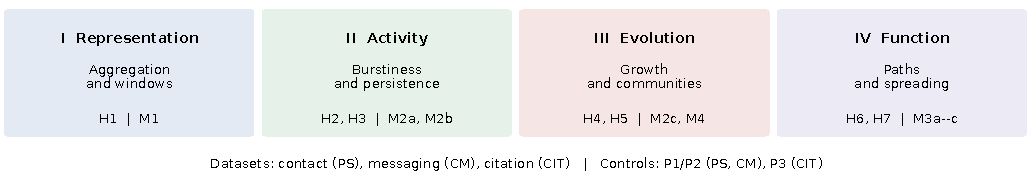
\includegraphics[width=\textwidth]{b_manuscript_framework.pdf}
\caption{Study design. Four aspects (Parts I--IV) map to seven hypotheses and four method
groups, in the order used throughout the paper. Reference models P1/P2 apply to PS and CM,
and P3 to CIT.}
\label{fig:framework}
\end{figure*}

\paragraph{Contributions.}
The study does not introduce new models. Its contribution is a question-driven synthesis of
the methods used to study temporal networks, a common and reproducible pipeline that applies
these methods to three types of empirical data, and a cross-network assessment of H1--H7
that identifies where temporal information is essential and where a static representation
suffices.

\paragraph{Organisation.}
\Cref{sec:related} reviews related work, \cref{sec:data} describes the data and
\cref{sec:methods} the methods. \Cref{sec:results} reports the results,
\cref{sec:discussion} discusses them and \cref{sec:conclusion} concludes.

%=====================================================================
\section{Related Work}
\label{sec:related}
The literature is organised by question, following Parts I--IV of the Introduction.
General frameworks and reviews are given by
\citet{holme2012temporal,holme2015modern} and the book of \citet{masuda2016guide}.
A central point of these reviews is that the basic unit is a \emph{contact}
(two nodes and a time), and that connectedness is no longer transitive: if $a$ meets
$b$ and later $b$ meets $c$, a path from $a$ to $c$ exists, but not the reverse path.
Consequently, a temporal network cannot be mapped onto a simple graph without losing
information or redefining its nodes, and many static-network methods require non-trivial
generalisations \citep{holme2015modern}.

\subsection{Representing time: aggregation, snapshots and windows}
\label{sec:rw-representation}
Temporal networks can be stored as contact sequences, interval graphs or sequences of
snapshots \citep{holme2012temporal}. Lossy representations such as weighted aggregates or reachability graphs reduce the
data to a static object; lossless ones keep all contacts \citep{holme2015modern}.
Each choice involves a trade-off: snapshots
make static tools applicable but require a window length, whereas the full event
sequence retains all information. The effect of this choice has been quantified for
communication data: window size and placement change the structure of the aggregated
network \citep{krings2012effects}, and coarser temporal resolution distorts
properties of the time-varying network in a way that depends on the system
\citep{ribeiro2013quantifying}. These findings motivate \textbf{H1}: aggregation and window
choice change structural conclusions.

\subsection{Temporal activity patterns}
\label{sec:rw-activity}
Human activity is bursty: inter-event times are heavy-tailed rather than exponential
\citep{barabasi2005origin}, and consecutive intervals are correlated, which
\citet{goh2008burstiness} capture with a burstiness coefficient and a memory
coefficient. Social ties are also repeated and persistent over long periods
\citep{saramaki2014persistence}, while the set of active links turns over. Temporal motifs
\citep{kovanen2011temporal,paranjape2017motifs} and activity-driven models
\citep{perra2012activity} describe and generate such patterns. These observations
motivate \textbf{H2} (activity is bursty and has memory) and \textbf{H3} (ties are repeated and
persistent while the network turns over).

\subsection{Structural evolution: growth, ageing and communities}
\label{sec:rw-evolution}
Growth is classically explained by preferential attachment
\citep{barabasi1999emergence}, whose strength can be measured directly from
growth data \citep{jeong2003measuring,newman2001clustering}. Real systems usually
show ageing, where old nodes attract fewer new links
\citep{dorogovtsev2000aging}, and in citations this is captured by a relevance
decay \citep{wang2013quantifying}. Growing networks also densify, with the number of
edges growing superlinearly in the number of nodes
\citep{leskovec2005graphs,leskovec2007graph}; node and link deletion alter these
laws \citep{moore2006exact}. These results motivate \textbf{H4}: growth follows preferential
attachment with ageing, and networks densify.

At the mesoscale, multilayer modularity couples partitions across time
\citep{mucha2010community}, communities can be tracked across snapshots through
matching \citep{greene2010tracking} and change can be mapped between partitions
\citep{rosvall2010mapping}; \citet{rossetti2018community} survey the field. Per-snapshot
partitions are typically obtained with Louvain \citep{blondel2008fast} or Leiden
\citep{traag2019louvain}. These methods motivate \textbf{H5}: communities reorganise over time and
a static partition hides this.

\subsection{Time and network function}
\label{sec:rw-function}
Because interactions occur in sequence, only time-respecting paths can carry
information: reachability in contact sequences is much lower than in the aggregated
graph \citep{holme2005network}, and path lengths and centrality change accordingly
\citep{pan2011path,kim2012temporal}. Burstiness and temporal correlations further
slow down spreading even when the static topology is unchanged
\citep{karsai2011small}. These results motivate \textbf{H6} (time ordering restricts
reachability and changes centrality rankings) and \textbf{H7} (burstiness and
temporal correlations slow down spreading).

\subsection{Randomized reference models}
\label{sec:rw-null}
Randomization is more versatile for temporal than for static networks, for which it is
essentially limited to degree-preserving link shuffling, because individual types of
correlation can be removed selectively \citep{holme2015modern}. Randomized reference models act as hypothesis tests: each one preserves some
properties of the data and destroys others, so differences between data and model
reveal which feature matters \citep{gauvin2022randomized}. Such models are used in
Parts II--IV (\cref{sec:null}).

\paragraph{Time scales and network types.}
Temporal networks are usually defined as systems whose evolution is not much slower
than the processes running on them, and a single system contains many time scales
(seconds, hours, days) \citep{holme2015modern}. Contact and communication data are
event sequences with such a hierarchy, whereas citation networks are acyclic by
construction and all out-links of a paper appear at one instant
\citep{holme2015modern}. Different network types are therefore expected to differ in
their sensitivity to temporal information.

\paragraph{Research gap.}
Most studies examine one dataset or one method, and few compare within a single
framework how sensitive different \emph{types} of networks are to temporal information.
The hypotheses distilled above (\cref{tab:hypotheses}) enable such a comparison.

%=====================================================================
\section{Data}
\label{sec:data}
One network is used per type. The three networks were chosen to differ in edge semantics,
generating mechanism and temporal resolution; their properties are summarised in
\cref{tab:data}.

\begin{table}[t]
\centering
\small
\setlength{\tabcolsep}{3pt}
\begin{tabular*}{\columnwidth}{@{\extracolsep{\fill}}llrrll@{}}
\toprule
Type & Dataset & $N$ & Events & Span & Res. \\
\midrule
Contact & Primary school (PS) & 242 & 125\,773 & 2 d & 20 s \\
Comm. & CollegeMsg (CM) & 1\,899 & 59\,798 & 193 d & 1 s \\
Citation & DBLP--DB (CIT) & 19\,150 & 73\,269 & 50 yr & 1 yr \\
\bottomrule
\end{tabular*}
\caption{Datasets. $N$: nodes; Res.: temporal resolution. CIT spans publication years
1970--2020; the primary analysis covers 1990--2020. PS is undirected and has class labels;
CM is directed and unlabelled; CIT is directed and acyclic.}
\label{tab:data}
\end{table}

\paragraph{Face-to-face contacts.}
The primary-school data \citep{stehle2011high,gemmetto2014mitigation} were collected by
the SocioPatterns collaboration with wearable proximity sensors over two school days. A
contact is recorded when two individuals are face to face within approximately 1.5\,m for
at least 20\,s. Each individual carries a class label, which serves as ground truth for
community detection. The data are released under CC BY-NC-SA 3.0. Activity is confined to
school hours (approximately 08:30--17:20), with up to 2,168 contact records per 10\,min and
no records overnight.

\paragraph{Online communication.}
CollegeMsg \citep{panzarasa2009patterns} contains time-stamped private messages between
1\,899 users of an online student community over 193 days at 1\,s resolution; removing
37 duplicate triples leaves 59,798 messages. Edges are directed, and no node labels are
available. Activity is strongly nonstationary: 37,680 messages (63\%) fall in May 2004, and
monthly volume declines steadily thereafter to 816 messages in October.

\paragraph{Scientific publications.}
The citation network is an induced subgraph of AMiner DBLP-Citation V14
\citep{tang2008arnetminer}, restricted to a fixed whitelist of database venues (SIGMOD,
VLDB/PVLDB, ICDE, PODS, EDBT, ICDT, TODS, VLDB Journal, Data \& Knowledge Engineering and
Information Systems) and their declared name variants. Of 5,259,858 streamed records,
19,150 publications from 1970--2020 are retained, including 6,709 isolates. A citation
$u\to v$ is dated by the publication year of $u$, and the primary graph requires
$y_v<y_u$; it contains 73,269 distinct citations and is therefore acyclic. The 5,486
same-year references, whose order cannot be resolved, are kept separately for a
sensitivity analysis; 6,390 references to later papers, 494 self-loops and 37,440
repeated reference entries are removed. Author self-citations are retained. All counts
refer to citations within the selected venues and not to global citation impact. AMiner
permits research use; no further licence is assumed. The number of retained citations per
year declines in the most recent years although the number of publications continues to
grow, which indicates coverage and censoring effects and motivates a sensitivity check
with a 2015 cutoff.

\paragraph{Preprocessing.}
All data are converted to a common event format $(u,v,t)$ with integer timestamps
(seconds or years) and a table of node labels. Self-loops and exact duplicate events are
removed. Each source has known limitations: the citation data have annual resolution,
the contact data cover only two days, and the sensors record only participating
individuals. The datasets differ by design in edge semantics (proximity, message,
citation), directedness and time scale, so that agreement across them cannot be
attributed to a single data type.

%=====================================================================
\section{Methods}
\label{sec:methods}
Every analysis follows the same template: hypothesis from the literature $\to$ metric
$\to$ randomized reference model. \Cref{tab:hypotheses} lists the seven hypotheses,
the methods (M1--M4) that test them and the datasets where each method is meaningful
(19 method--dataset pairs). The empty cells are deliberate: CIT is a year-resolution
DAG without fine-grained events (no M2a, M2b, M3) and without community
reorganisation (no M4), while PS and CM have no growth process (no M2c).

\begin{table*}[t]
\centering
\small
\setlength{\tabcolsep}{4pt}
\begin{tabular*}{\textwidth}{@{\extracolsep{\fill}}cl p{8cm} l l l ccc@{}}
\toprule
Part & ID & Hypothesis & Source & Method & Null & PS & CM & CIT \\
\midrule
I   & H1 & Aggregation and window choice change structural conclusions
           & \citep{krings2012effects,ribeiro2013quantifying} & M1 & -- & \checkmark & \checkmark & \checkmark \\
\midrule
II  & H2 & Activity is bursty and has memory
           & \citep{goh2008burstiness} & M2a & P1 & \checkmark & \checkmark & \\
    & H3 & Ties are repeated and persistent; the network turns over
           & \citep{saramaki2014persistence} & M2b & P1 & \checkmark & \checkmark & \\
\midrule
III & H4 & Growth follows preferential attachment with ageing; networks densify
           & \citep{jeong2003measuring,wang2013quantifying,leskovec2005graphs} & M2c-1--4 & P3 & & & \checkmark \\
    & H5 & Communities reorganise over time; the static partition hides this
           & \citep{greene2010tracking,mucha2010community} & M4 & P1 & \checkmark & \checkmark & \\
\midrule
IV  & H6 & Time ordering restricts reachability and changes centrality rankings
           & \citep{holme2005network,pan2011path,kim2012temporal} & M3a, M3b & P1, P2 & \checkmark & \checkmark & \\
    & H7 & Burstiness and temporal correlations slow down spreading
           & \citep{karsai2011small} & M3c & P1, P2 & \checkmark & \checkmark & \\
\bottomrule
\end{tabular*}
\caption{Hypotheses tested in this work, with methods, null models
(\cref{sec:null}) and applicable datasets.}
\label{tab:hypotheses}
\end{table*}

\subsection{Notation}
\label{sec:notation}
Let $\mathcal{E}=\{(u,v,t)\}$ be the event sequence. The static aggregate $G$
contains a link $(u,v)$ if at least one event occurs between $u$ and $v$. A
snapshot $G_{\Delta t}(k)$ contains the events in $[k\Delta t,(k+1)\Delta t)$, and the
cumulative network $G(\le t)$ contains all events up to $t$.

\subsection{Aggregation and time windows (M1)}
\label{sec:m-aggregation}
For each window length $\Delta t$ on a grid (PS: 5\,min to 1\,day; CM: 1\,h to 1\,month)
we compute density, mean degree, clustering coefficient and giant-component size of the
snapshots and of the aggregate. For CIT, yearly and cumulative networks are compared.
\emph{Window sensitivity} is the relative change of a metric across the grid.
Rankings are handled separately in M3b. Aggregation can introduce paths that
cannot be traversed in time: if $c$--$d$ occurs before $a$--$b$ and $b$--$c$,
the static path $a$--$b$--$c$--$d$ is not time-respecting from $a$.




\subsection{Activity patterns (M2a, M2b)}
\label{sec:m-activity}

\textbf{M2a: Burstiness and memory.}
We analyse inter-event times for each interacting node pair
in the Primary School (PS) and CollegeMsg (CM) networks.
PS contacts are recorded every 20 seconds. Consecutive
records for the same unordered pair, separated by exactly
20 seconds, are merged into a single contact episode.
For CM, each retained directed message is treated as
an independent event.

For each edge, inter-event intervals are calculated
from consecutive event timestamps. We pool these
intervals across edges and calculate burstiness as
\begin{equation}
B = \frac{\sigma-\mu}{\sigma+\mu},
\end{equation}
where $\mu$ and $\sigma$ are the mean and population
standard deviation of the pooled intervals.

Memory is defined as the Pearson correlation between
consecutive inter-event intervals within each edge,
pooled across all valid adjacent interval pairs
\citep{goh2008burstiness}.
Both $B$ and $M$ are pooled statistics rather than
averages of per-edge coefficients.

\textbf{M2b: Repetition, lifetime and turnover.}
We quantify temporal link persistence using three metrics.

The repetition rate is the fraction of distinct edges
with at least two independent contact episodes (PS)
or two messages (CM).

Edge lifetime is defined as the difference between
the last and first event timestamps of each edge.
Edges observed only once have zero lifetime.

Link turnover is measured using the Jaccard similarity
between edge sets in consecutive time windows:
\begin{equation}
J(E_k,E_{k+1}) =
\frac{|E_k \cap E_{k+1}|}
{|E_k \cup E_{k+1}|}.
\end{equation}
We average this quantity over adjacent window pairs
with nonempty unions.

The default window size is one hour for PS and
seven days for CM. We additionally evaluate
15, 30, 60 and 120-minute windows for PS,
and 1, 3, 7 and 14-day windows for CM.

For PS, edge lifetime and window Jaccard are computed
from the original event stream. We also compare raw
20-second records with merged contact episodes
to assess the sensitivity of H2 to event definition.


\subsection{Structural evolution (M2c, M4)}
\label{sec:m-evolution}
% Owner: B (expanded M2c-1 through M2c-4 and P3).
\paragraph{M1 for citations.}
Annual and cumulative citation networks share the same node set at year $t$, namely all
selected papers published by $t$. Directed density is $E/[N(N-1)]$ and mean total degree
is $2E/N$; clustering, component counts and LCC fractions use the weak undirected
projection, including isolates. Trailing windows of 1, 2, 5 and 10 years provide the
window grid. Window sensitivity, $(\max-\min)/\mathrm{mean}$ over the grid, is computed at
each end year and averaged over end years 1990--2020, which constitute the primary
analysis interval; earlier papers enter as history.

\paragraph{M2c-1: preferential attachment.}
Following the degree-class approach of \citet{jeong2003measuring}, in-degrees are frozen
at the start of each citing year, and for each prior-degree class $k$ the number of
eligible papers $n_{tk}$ and of new citations $h_{tk}$ are counted. The exponent $\alpha$
is estimated by conditional likelihood with target probabilities proportional to
$n_{tk}(k+1)^\alpha$, conditioning on the total number of citations in each year. The
offset admits citations to previously uncited papers; offsets of 0.5 and 2 serve as
sensitivity checks. Confidence intervals use 400 bootstrap resamples of citing-year blocks
and are descriptive. Neither a positive $\alpha$ nor its departure from an age-only
reference identifies a causal mechanism.

\paragraph{M2c-2: ageing.}
For ages 1--60, the target probability in citing year $t$ is proportional to
$n_{ta}f(a)$, where $n_{ta}$ is the number of available papers of age $a$. Lognormal,
exponential, power-law and uniform kernels $f$ are compared by AIC on identical
observations and support. The comparison is repeated by publication cohort (1970--1989,
1990--1999, 2000--2009), accounting for each cohort's exposure. The estimate describes
marginal ageing, which may also reflect degree, fitness and venue coverage.

\paragraph{M2c-3: densification and diameter.}
The densification exponent $a$ is obtained from $\log E(t)=a\log N(t)+b$ over 1990--2020
and over split periods and an earlier cutoff. Year-resampling intervals are descriptive
because cumulative observations are dependent. The effective diameter is the 90th
percentile of shortest-path distances within the largest weak component, estimated from
128 uniformly sampled source nodes per year, with 64 and 256 sources as sensitivity checks
\citep{leskovec2005graphs}.

\paragraph{M2c-4: citation dynamics and prediction.}
The Wang--Song--Barab\'asi (WSB) model \citep{wang2013quantifying},
\begin{equation}
 c(t)=m\left[\exp\!\left\{\lambda\Phi\left(\frac{\log t-\mu}{\sigma}\right)\right\}-1\right],
\end{equation}
is fitted with $m$ fixed to the mean within-subgraph reference count of papers published
up to 1989. Bounded multistart least squares minimizes the squared error of $\log(1+c)$;
parameter bounds and boundary flags are recorded. Descriptive fits use a random sample of
at most 500 papers published in 1990--2005 with at least 10 citations by age 15, fitted
over ages 1--15; the resulting collapse is in-sample evidence only. For prediction,
papers are selected using only their first five years (at least five citations by age
five; random sample of at most 500), and WSB is compared with a no-ageing preferential
attachment baseline, $c(t)=m[\exp(rt)-1]$, and with linear extrapolation, $c(5)t/5$. The
primary task predicts cumulative citations at age 15, which is observed for every selected
paper; a secondary task predicts the 2020 total with a variable horizon. Neither target
represents lifetime citations. This fixed-horizon design differs from the original study,
which trains on 5 or 10 years and evaluates at age 30 \citep{wang2013quantifying}.
Performance is measured by mean absolute error (MAE), median absolute error and root mean
squared logarithmic error (RMSLE), with paired bootstrap differences (1000 resamples). Fits
at a parameter bound remain in the primary evaluation, and an interior-fit subset serves
as a sensitivity check; a constrained optimum is not regarded as a convergence failure.

\paragraph{P3: citation-target randomization.}
Twenty realizations per model preserve each paper's publication year and its number of
distinct references, which are drawn without replacement from strictly older papers. P3a
selects targets uniformly. P3b weights targets by a nonparametric age kernel fitted by
conditional likelihood to the observed data and removes degree preference. Because P3b is
calibrated on the data, its agreement with the observed ageing is not independent
confirmation. Null means and sample standard deviations are reported; empirical tail
probabilities have a resolution of $1/21$. Both models fix $N(t)$ and $E(t)$ and thus
preserve the densification exponent exactly; they test diameter and target preference but
not densification itself.


\textbf{M4} detects communities in every snapshot (Leiden or Louvain), matches them
across snapshots \citep{greene2010tracking} and reports modularity and the number of
communities over time, the normalised mutual information (NMI) between consecutive
snapshots, the NMI between the dynamic and the static partition, and for PS the NMI
with the class labels. The resolution parameter is fixed and its effect is checked.

\subsection{Paths, centrality and spreading (M3)}
\label{sec:m-function}
\textbf{M3a} computes earliest-arrival time-respecting paths and the temporal reachability
ratio $R$ (fraction of node pairs connected by a time-respecting path, relative to the
static aggregate). \textbf{M3b} compares static and temporal closeness rankings by
Kendall's $\tau$. \textbf{M3c} runs an event-driven SIR process on the event sequence with
at least 100 random seeds; SI with certain transmission is equivalent to M3a, so only SIR
is run.


\subsection{Randomized reference models}
\label{sec:null}
No single temporal counterpart of the configuration model exists, so one switches off
selected correlations with different models and compares the outcomes
\citep{holme2012temporal,gauvin2022randomized}.

For PS and CM, we consider two complementary types of randomization,
corresponding to \emph{randomly permuted times} (RP) and
\emph{randomized edges} (RE) in the naming of
\citet{holme2012temporal}.

\textbf{P1 (RP): Timestamp permutation.}
P1 randomly permutes timestamps among events while keeping their
endpoints unchanged. It preserves the static graph, the number of
contacts of every pair, and the global timestamp distribution,
while disrupting the original temporal correlations.
For H2 and H3, we generate 20 realizations and report
the null mean and standard deviation.

\textbf{P2: Structural randomization.}
We distinguish two variants of edge randomization.

\textbf{P2a (RE, original proposal).}
The original method rewires the static graph in a
degree-preserving way while each pair's contact sequence
moves with its link. It aims to destroy the wiring diagram
while preserving per-link temporal activity patterns
and the overall event rate.
This variant is retained as the original methodological
proposal but was not evaluated in the Member C experiments.

\textbf{P2b (constrained endpoint swaps, implemented).}
Our implementation randomly swaps endpoints between event pairs
while keeping timestamps fixed. For undirected PS, endpoint
orientations are randomized before swapping; for directed CM,
sender and receiver roles are preserved. Swaps creating self-loops
or duplicate edge-time events are rejected.

P2b preserves the total event count, timestamp multiset,
and node event participation counts (separate sender and
receiver counts for CM). Unlike P2a, it does not necessarily
preserve static simple-graph degrees or individual edge
contact sequences.

We attempt five swaps per event and validate the structural
invariants using a fixed random seed of 42.
These checks do not establish uniform sampling or sufficient
mixing of the randomization process.

Comparing temporal and structural randomization helps
distinguish the effects of event timing from network topology.
Combined models (RE+RP) and fully random times (RT)
remain possible extensions.


\subsection{Measuring the effect of time}
\label{sec:time-effect}
Raw metrics cannot be compared across a contact network, a message network and a
citation network, so we define one normalised measure per hypothesis:
H1 window sensitivity (relative change of a metric over the $\Delta t$ grid);
H2 differences in pooled burstiness and memory
relative to P1,
$B_{\mathrm{real}}-\overline{B}_{\mathrm{P1}}$
and
$M_{\mathrm{real}}-\overline{M}_{\mathrm{P1}}$;
H3 differences in adjacent-window link Jaccard
relative to P1,
$J_{\mathrm{real}}-\overline{J}_{\mathrm{P1}}$;
H4 exponents $\alpha$ and $a$;
H5 mean consecutive-snapshot NMI and dynamic-vs-static NMI;
H6 reachability ratio $R$ and Kendall $\tau$(static, temporal);
H7 slowdown $T_{\mathrm{real}}/T_{\mathrm{null}}$, where $T$ is the time to the epidemic peak.

\subsection{Implementation}
All code is in Python. We use NetworkX for static graph analysis, Raphtory
\citep{steer2024raphtory} for time-respecting paths, tnetwork for dynamic communities,
and Leiden/Louvain for per-snapshot partitions. Null models, the attachment-kernel
estimator and the SIR process are custom code, unit-tested on hand-built examples
whose answers are known (reachability, SIR, preserved quantities of P1 and P2). Random
seeds are fixed and every figure is generated by one script.

\section{Results}\label{sec:results}
The results follow the four method groups. All primary PS/CM cells now contain
measurements; null comparisons use 20 networks per family. The supplementary
robustness tables retain individual networks and elapsed-time half-window results.
\subsection{Aggregation and time windows}
\label{sec:r-aggregation}

% Owner: A
\paragraph{Contact and messaging networks (PS, CM).}
\outline{Which conclusions are stable under window choice, and over which
$\Delta t$ range?}
\expect{[Expected] Density and clustering of the snapshots rise quickly with
$\Delta t$ and approach the aggregate only for windows comparable to the whole
observation period. The giant component of short-window snapshots is small, and
percolates at a window that is much shorter for CM than for PS because PS has a
daily rhythm (lessons, breaks). Conclusions about ``the'' clustering or density of
the network therefore depend strongly on $\Delta t$.}

% PS/CM plots await measured results; no empty figure is reserved.


% Owner: B
% Owner: B -- measured CIT contribution only.
\paragraph{Citation network (CIT).}
In 2020, annual and cumulative graphs on the same 19,150 born nodes contain
1,450 and 73,269 citations. Mean total degree is 0.151 versus 7.652, weak
largest-component fraction 0.052 versus 0.641, and cumulative weak clustering
0.124. Annual clustering is identically zero: strict older-target citations make
each annual snapshot bipartite. This is a consequence of the representation,
not independent evidence for temporal correlations. Over 1-, 2-, 5- and 10-year
windows, relative ranges average 1.798 for density/degree, 2.361 for clustering
and 1.114 for largest-component fraction.
\textbf{CIT verdict on H1:} window choice changes structural descriptions;
some differences are definitional. The node denominator and year convention
must accompany every comparison.



\paragraph{Window interpretation.}
\Cref{fig:b-aggregation}(c,d) shows that longer windows connect a larger fraction of born
papers and admit cross-year triangles. These effects require a sequence of
snapshots; one final aggregate cannot reveal when connectivity appears.
The relative range is a window-sensitivity statistic, not a significance test
against a temporal null, and identical density/degree sensitivity follows from
the common denominator.



\begin{figure*}[t]
\centering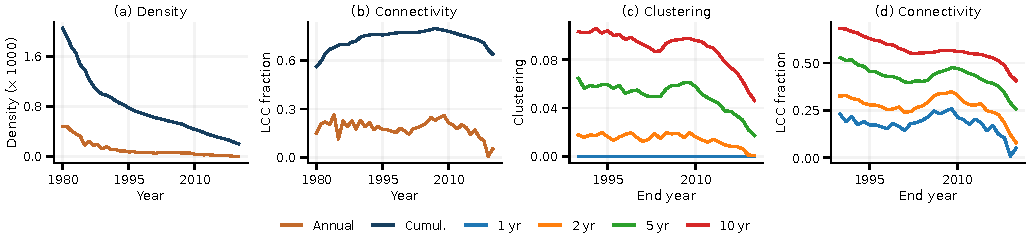
\includegraphics[width=\textwidth]{b_manuscript_aggregation.pdf}
\caption{CIT representation effects. (a,b) Annual versus cumulative density and
weak-LCC fraction; (c,d) clustering and connectivity for 1-, 2-, 5- and 10-year
trailing windows. All fractions include born isolates. Annual zero clustering
follows from strict publication-year ordering; it is not separate mechanism evidence.}
\label{fig:b-aggregation}
\end{figure*}


\paragraph{Verdict on H1.}
Supported for CIT under the stated node denominator and strict-year convention.
A comparative verdict for PS and CM awaits their measurements; the relative
sensitivity of network types cannot yet be ranked.

\subsection{Activity patterns (H2, H3)}\label{sec:r-activity}
\Cref{tab:burst} compares the activity statistics of both networks with P1.

\begin{table}[t]
\centering\small
\begin{tabular*}{\columnwidth}{@{\extracolsep{\fill}}llrr@{}}
\toprule Network & Metric & Real & P1 mean $\pm$ SD \\
\midrule
PS & $B$ & 0.535 & $0.5184\pm0.0004$ \\
PS & $M$ & 0.020 & $0.0710\pm0.0016$ \\
PS & Repeated ties & 0.625 & $0.6568\pm0.0001$ \\
PS & Jaccard & 0.220 & $0.3668\pm0.0010$ \\
CM & $B$ & 0.581 & $0.2451\pm0.0012$ \\
CM & $M$ & 0.100 & $0.2288\pm0.0057$ \\
CM & Repeated ties & 0.495 & $0.4949\pm0.0000$ \\
CM & Jaccard & 0.096 & $0.0690\pm0.0009$ \\
\bottomrule\end{tabular*}
\caption{Burstiness $B$, memory $M$, repeated-tie fraction and adjacent-window Jaccard
similarity (1-h windows for PS, 7-day windows for CM). The CM repeated-tie fraction is
invariant under P1 and therefore descriptive.}\label{tab:burst}
\end{table}

\paragraph{Burstiness and memory (H2).}
Burstiness exceeds the P1 value in both networks, by $\Delta B=+0.016$ in PS and $+0.336$
in CM, whereas memory is lower than under P1 in both ($\Delta M=-0.051$ and $-0.129$). The
PS excess is small in absolute terms over the full interval, although large relative to
the narrow null dispersion; it increases to $+0.116$ and $+0.120$ in the two single-day
halves (real/null 0.404/0.288 and 0.395/0.275). The inactive night between the two school
days is a plausible contributor but cannot be isolated with these data. The mean tie
lifetime is 0.444 days against 0.690 days under P1 in PS, and 4.756 days against 30.028
days in CM.

\paragraph{Persistence and turnover (H3).}
Adjacent-window similarity is lower than under P1 in PS ($\Delta J=-0.147$), indicating
rapid turnover of the contact set. In CM the full-period similarity exceeds that of P1
($\Delta J=+0.027$), but the sign reverses within both halves (0.074 against 0.113 and 0.118
against 0.140). The CM contrast thus depends on the observation interval: P1 redistributes
timestamps over the selected interval, so its baseline varies with the duration, activity
level and window composition of that interval, and the present comparison does not identify
which of these factors is responsible. The repeated-tie fraction of CM is invariant under
P1 by construction and serves only as a description.

\paragraph{Verdict on H2 and H3.}
H2 is supported for burstiness, with an interval-dependent magnitude in PS and a large
effect in CM, and is not supported for memory, which is weaker than under P1 in both
networks. For H3, PS shows rapid turnover, whereas the CM persistence contrast depends on
the observation interval and does not support a general claim of more persistent ties.

\subsection{Structural evolution (H4, H5)}\label{sec:r-evolution}
\subsubsection{Growth, ageing and densification of the citation network (H4)}
\paragraph{Preferential attachment (H4a).}
The conditional attachment kernel $(k+1)^\alpha$ yields $\alpha=0.714$ with a descriptive
95\% year-bootstrap interval $[0.693,0.730]$ (\cref{fig:growth}a). Twenty P3a samples give
$0.0006\pm0.0051$ and the age-only control P3b gives $-0.6512\pm0.0053$
(\cref{fig:growth}b); the observed exponent exceeds all null values, corresponding to an
empirical one-sided probability of $1/21$ per comparison. The exponent remains positive
under time splits, degree offsets of 0.5 and 2, and a core subset of venues
(\cref{sec:r-robustness}). Sublinear degree preference is therefore supported within this
corpus beyond the age-only reference, without identifying a causal attachment mechanism.

\begin{figure*}[t]
\centering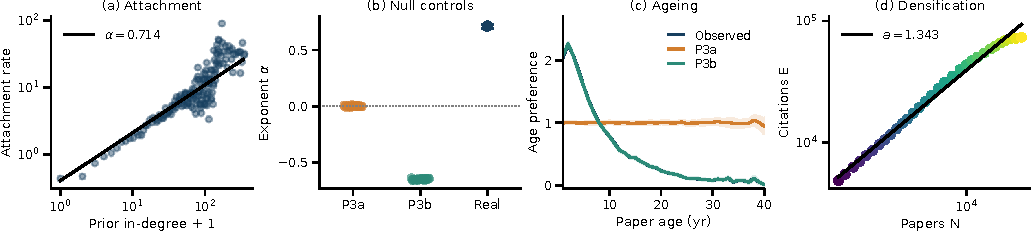
\includegraphics[width=\textwidth]{b_manuscript_growth.pdf}
\caption{CIT growth mechanisms. (a) Attachment rate by prior-degree class (classes with at
least five citations); the line shows the fitted exponent. (b) Exponents of 20 samples per
reference model and the observed exponent with its year-bootstrap interval. (c)
Exposure-adjusted age preference (null mean $\pm$ SD). (d) Cumulative edge count against
node count, 1990--2020.}
\label{fig:growth}
\end{figure*}

\paragraph{Ageing (H4b).}
A lognormal age kernel is preferred over exponential, power-law and uniform kernels
(\cref{tab:b-age-models}). The fitted parameters are $(\mu,\sigma)=(1.858,1.108)$,
corresponding to a scale $e^\mu$ of 6.41 years. The mean age of cited papers is 5.711
years, against $11.457\pm0.034$ under P3a and $5.717\pm0.018$ under the calibrated control
P3b (\cref{fig:growth}c). The lognormal kernel is preferred in all three publication
cohorts, although the tails of the most recent cohort remain censored. Age-independent
target choice is therefore rejected; the agreement of P3b follows from its calibration and
does not constitute independent confirmation.

\begin{table}[t]
\centering\small
\setlength{\tabcolsep}{4pt}
\begin{tabular*}{\columnwidth}{@{\extracolsep{\fill}}lrr@{}}
\toprule Age kernel & Parameters & $\Delta$AIC\\
\midrule
Lognormal & 2 & 0.0\\
Exponential & 1 & 537.8\\
Power-law & 1 & 9,360.5\\
Uniform & 0 & 41,796.7\\
\bottomrule
\end{tabular*}
\caption{CIT age-preference kernels fitted on identical observations. AIC selects among
the stated models and not among all possible ageing mechanisms.}
\label{tab:b-age-models}
\end{table}

\paragraph{Densification and diameter (H4c).}
For 1990--2020 the densification exponent is $a=1.343$ ($R^2=0.991$) with a descriptive
year-resampling interval $[1.288,1.406]$ (\cref{fig:growth}d). Densification is weaker in
2005--2020 ($a=1.065$) than in 1990--2004 ($a=1.455$). Here densification denotes
superlinear growth of the edge count and not increasing directed density. The effective
diameter of the largest weak component equals 6 hops in every year and is unchanged with
64 or 256 source nodes, so no shrinkage is detected at this resolution. Because P3 fixes
$N(t)$ and $E(t)$, it preserves $a$ by construction and cannot test densification.

\paragraph{Citation dynamics and prediction (H4d).}
For 500 full-history fits, the median WSB parameters are
$(\lambda,\mu,\sigma)=(2.717,0.834,1.238)$, with median RMSLE 0.074 and scaled-collapse RMSE
0.022; these are in-sample diagnostics. In the held-out task (\cref{tab:b-forecast}), WSB
predicts cumulative citations at age 15 with an MAE of 15.144, against 17.064 for linear
extrapolation. The paired difference (WSB minus linear) has a 95\% bootstrap interval of
$[-4.471,0.806]$ at age 15 and $[-4.764,8.128]$ for the 2020 total; both intervals contain
zero. The no-ageing baseline over-extrapolates by several orders of magnitude, so
outperforming it alone is a weak test. Forecast fits reach a parameter bound for 193 of 500
papers (38.6\%), although all optimizations report success; boundary solutions reflect limited
identifiability in short histories rather than optimizer failure. Compact descriptive fits
are thus supported, whereas a predictive advantage over linear extrapolation is not
established.

\begin{table}[t]
\centering\small
\setlength{\tabcolsep}{4pt}
\begin{tabular*}{\columnwidth}{@{\extracolsep{\fill}}llrr@{}}
\toprule Target & Model & MAE & RMSLE\\
\midrule
Age 15 & WSB & 15.144 & 0.601\\
 & Linear & 17.064 & 0.662\\
 & No-ageing PA & 27,588 & 4.601\\
\midrule
2020 & WSB & 28.016 & 0.778\\
 & Linear & 27.271 & 0.876\\
 & No-ageing PA & $2.79\!\times\!10^6$ & 7.000\\
\bottomrule
\end{tabular*}
\caption{Citation forecasts for 500 papers trained on years 1--5. Age 15 is the primary,
fixed-horizon target; the 2020 total is a secondary target with variable horizon.}
\label{tab:b-forecast}
\end{table}

\paragraph{Verdict on H4.}
Sublinear preferential attachment, age-dependent target choice and superlinear edge growth
are supported within this corpus, whereas diameter shrinkage and a forecast advantage of the
WSB model are not. All counts are restricted to the selected venues.

\subsubsection{Dynamic and static communities (H5)}
\paragraph{Primary school.}
Outside the midday break, snapshot communities closely match the classes (NMI
$\approx 0.85$--$0.95$), as does the static partition (six communities, NMI 0.86 with the
classes; \cref{fig:m4-ps}). Between approximately 12:00 and 14:00 on both days, the NMI with
the classes and with the static partition falls to $\approx 0.5$. Under P1 both curves remain
flat (class NMI $0.86\pm0.002$), so the decline is attributable to the timing of contacts
and not to the identity of the contacting pairs. Nor is it algorithmic noise: two Leiden runs
on the same window agree with NMI 0.98 on average. Averaged over the day, real snapshots agree
less with the static partition than P1 snapshots (0.72 against $0.94\pm0.003$).

\begin{figure*}[t]
\centering
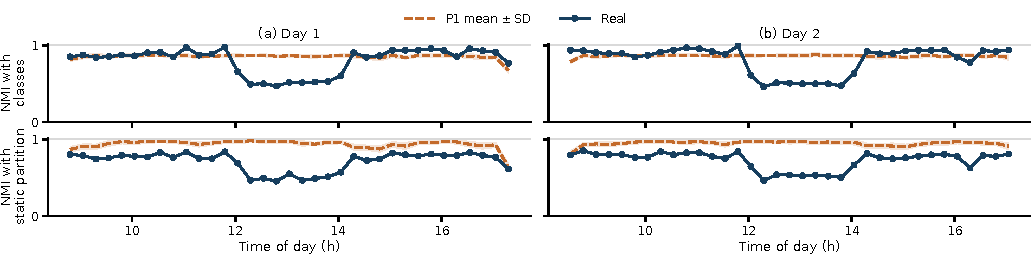
\includegraphics[width=\linewidth]{e_m4_ps_timeseries.pdf}
\caption{Snapshot communities in PS (15-min windows, $\gamma=1$): NMI with the classes (top)
and with the static partition (bottom). P1: mean $\pm$ SD of 20 samples.}
\label{fig:m4-ps}
\end{figure*}

\paragraph{CollegeMsg.}
Weekly snapshots agree only weakly with each other and with the static partition (NMI 0.52
and 0.34), and P1 yields similar values (0.42 and 0.32). Snapshots are sparse, with on
average 326 of 1,899 users active per week, and during the first two months two runs of
the algorithm on the same window agree only at NMI $\approx 0.65$--$0.7$. Where real and
null values differ, real snapshots resemble their predecessor more than randomized
snapshots do, which indicates persistent conversation groups rather than reorganisation.
This community-level result is distinct from the tie-level overlap of \cref{sec:r-activity}.

\paragraph{Sensitivity.}
The comparison was repeated for three window widths and three resolutions $\gamma$. In PS,
real snapshots agree less with the static partition than P1 snapshots in all nine settings
(differences between $-0.03$ and $-0.23$). In CM the difference remains within $\pm0.06$,
and within $\pm0.025$ except for 30-day windows with $\gamma=0.5$. The comparison with the
previous window is not robust in PS: at 15 and 60\,min real snapshots change more than P1
snapshots, whereas at 5\,min the order reverses, because a 5-min P1 snapshot is a small
random sample of the static graph. Larger $\gamma$ yields more and smaller communities
without changing these signs. Timestamp permutation spreads each node's events over the
whole period, so a P1 window contains almost all nodes (240 against 175 active nodes per
15-min PS window); part of the gap to the static partition therefore reflects which nodes
are active at a given time, in addition to which nodes interact. The midday decline of the
class NMI is unaffected, because it compares real snapshots with external labels.

\paragraph{Verdict on H5.}
H5 is supported for face-to-face contacts and not supported for online messages. In PS the
static partition recovers the classes but conceals the midday mixing, which P1 does not
reproduce. In CM the static partition summarises the weekly snapshots as well as it
summarises time-shuffled ones, and the snapshots are, if anything, more persistent than
random.

\subsection{Paths, centrality and spreading}\label{sec:r-function}
% Owner: D
% M3a - Temporal Reachability

\begin{figure}[t]
    \centering
    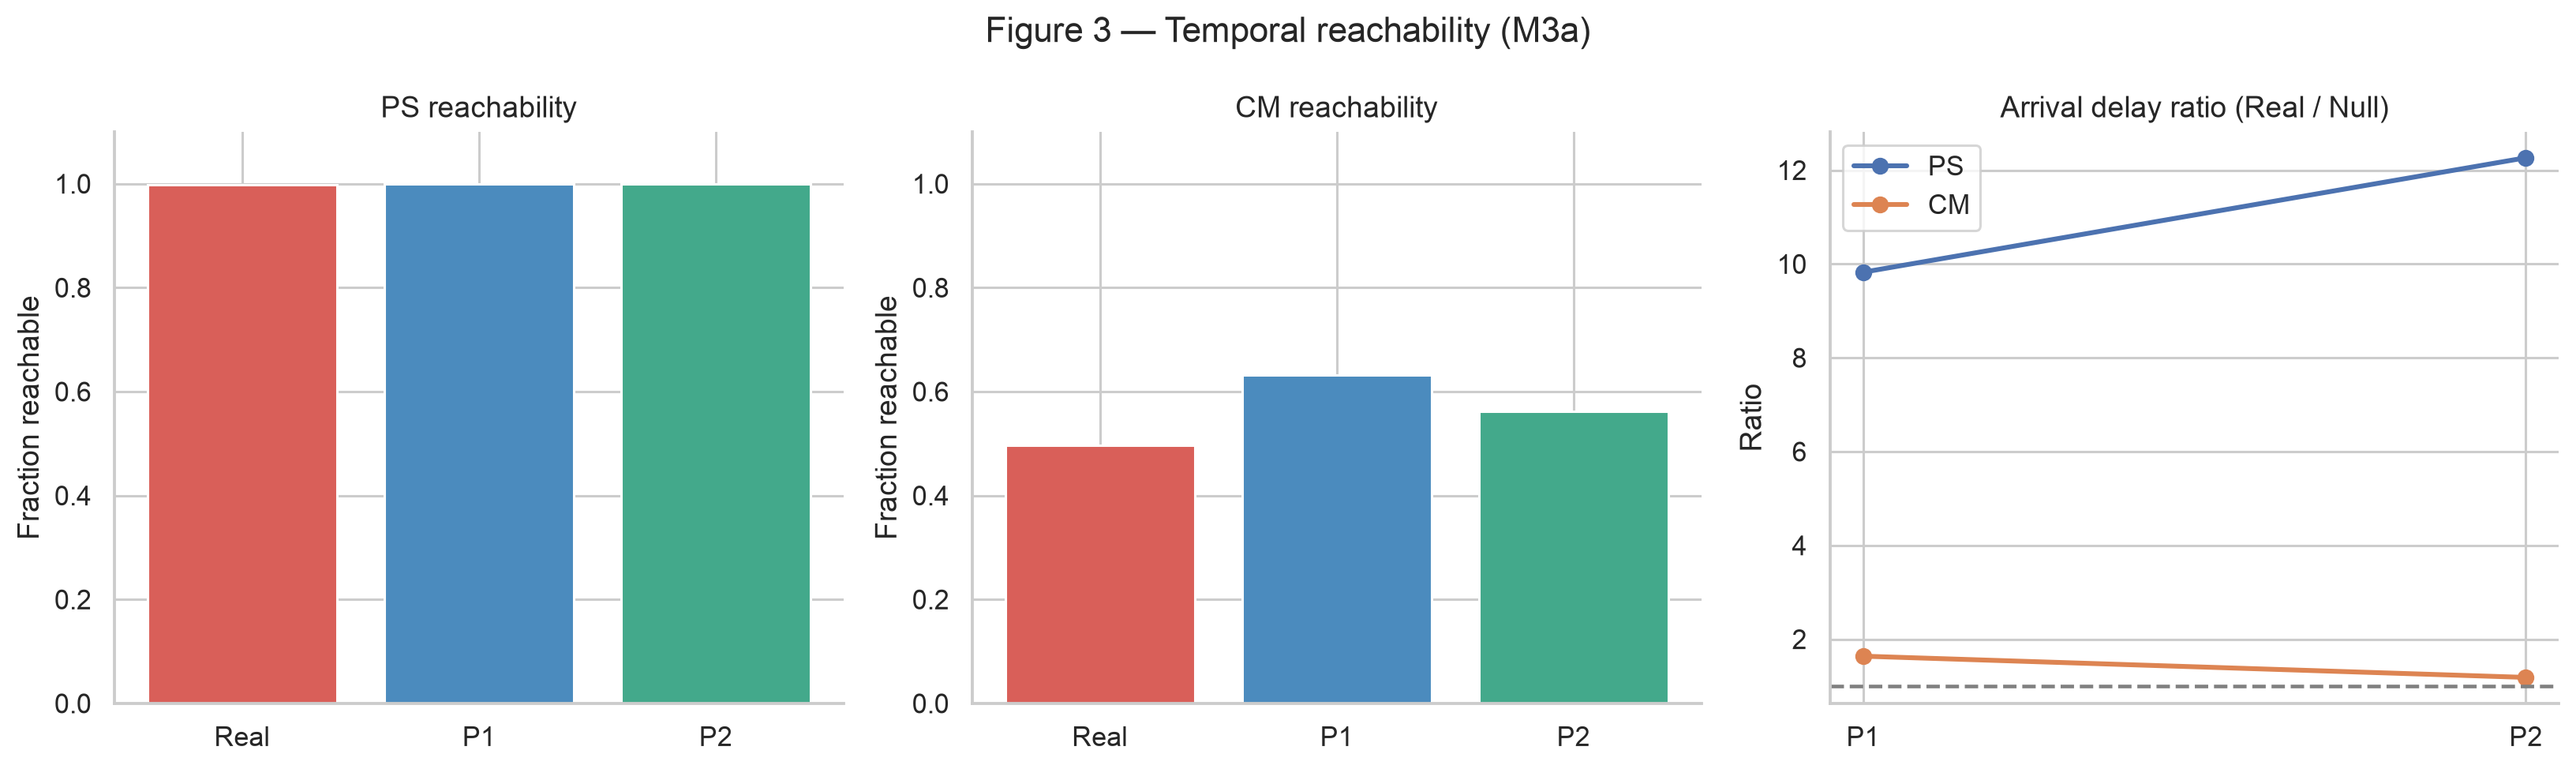
\includegraphics[width=\linewidth]
    {Fig3_reachability_and_delay.png}
    \caption{Temporal reachability comparison
    between real and randomized networks.}
    \label{fig:d_reachability}
\end{figure}

% 后面继续放你的完整M3a实验分析
% =========================================================
% Member D: M3a Temporal Reachability and M3c SIR Spreading
% =========================================================

\subsubsection{Temporal Reachability (M3a)}
\label{sec:d_reachability}

We first investigate H6a: temporal ordering restricts
network reachability. We compare the original temporal
networks (Real) with timestamp-shuffled (P1) and
edge-randomized (P2) reference networks.

Two metrics are considered: temporal reachability and
mean earliest-arrival delay. The former measures the
fraction of reachable nodes under time-respecting paths,
while the latter measures the time required to reach
accessible destinations.

\paragraph{Reachability results.}

Figure~\ref{fig:d_reachability} presents the temporal
reachability results for the Primary School (PS) and
CollegeMsg (CM) datasets.

\begin{figure*}[t]
    \centering
    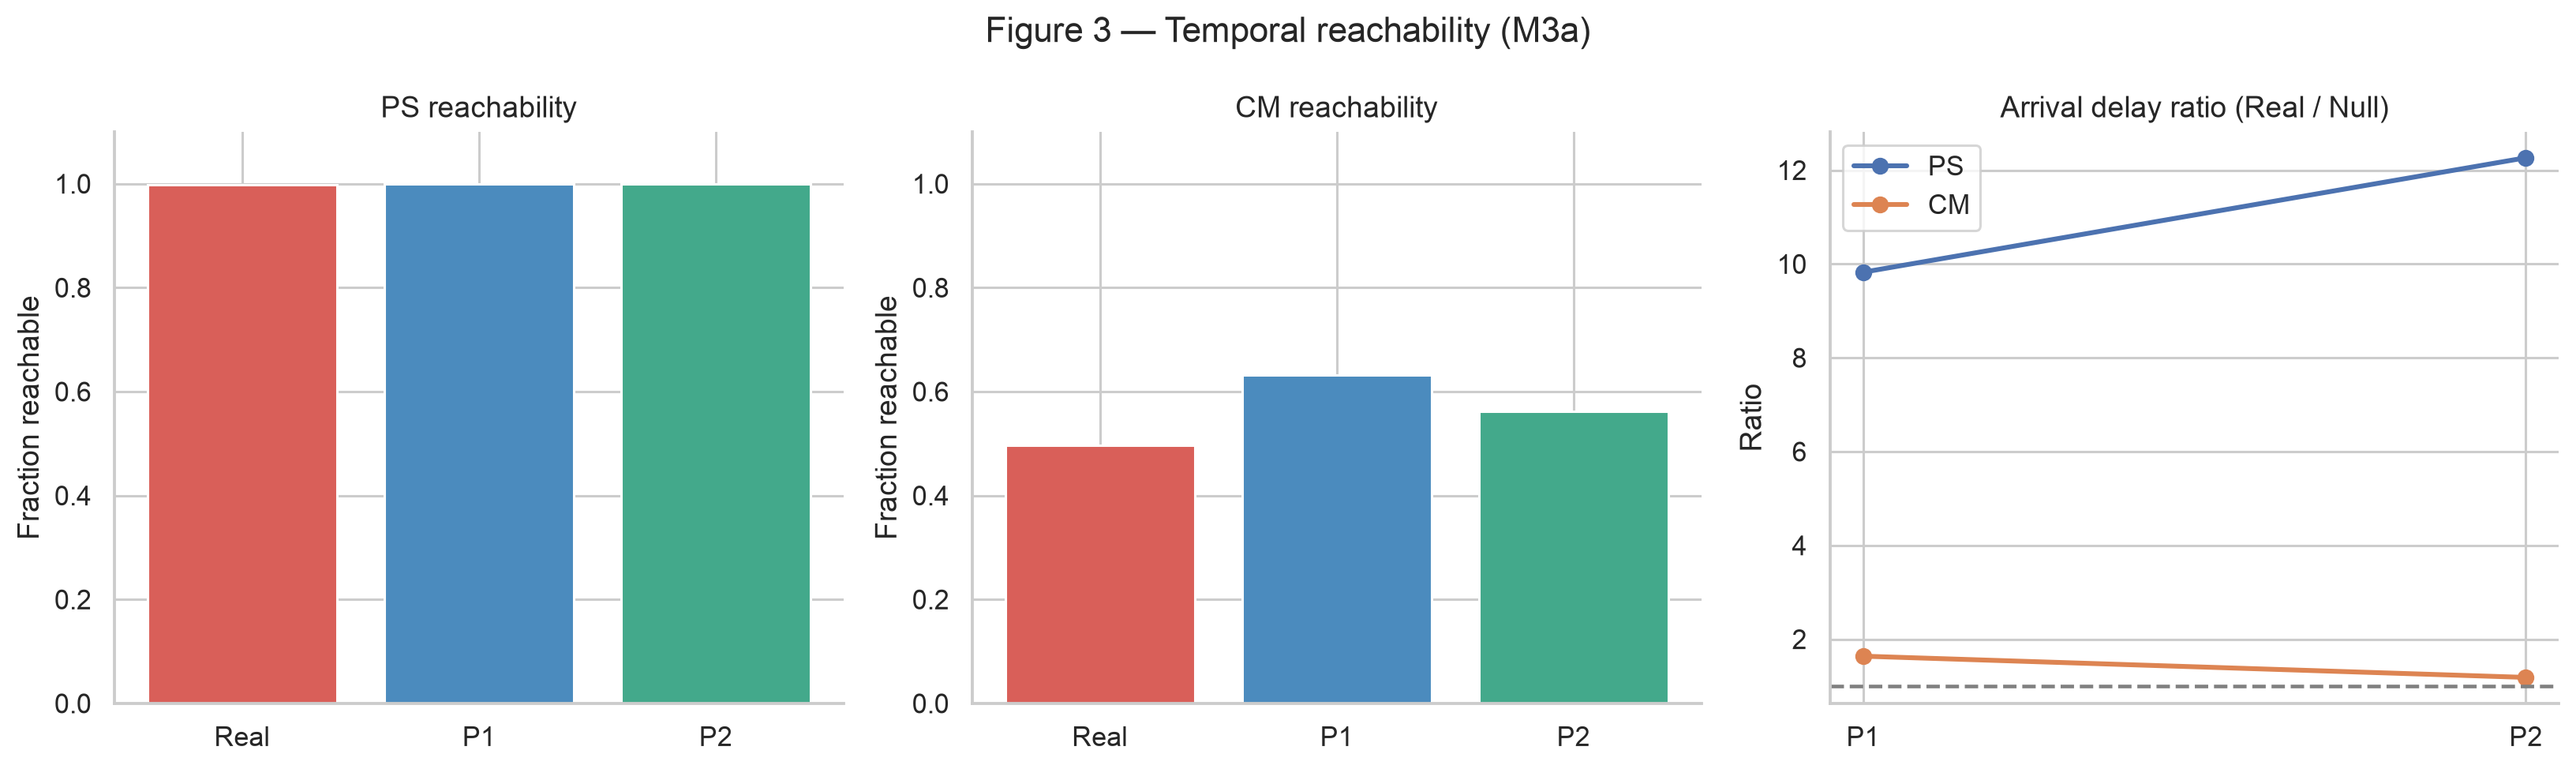
\includegraphics[width=0.85\textwidth]
    {Fig3_reachability_and_delay.png}
    \caption{Temporal reachability analysis (M3a).
    The first two panels show reachability in PS and CM.
    The third panel compares the real-to-null arrival-delay
    ratios. Ratios above one indicate longer arrival delays
    in the original temporal network.}
    \label{fig:d_reachability}
\end{figure*}

In PS, the real network achieves a reachability ratio
of 0.9981, compared with 1.0000 for both P1 and P2.
Thus, almost all nodes remain temporally reachable
regardless of randomization.

However, the mean arrival delay differs substantially.
The real-network delay is approximately 9.82 times
that of P1 and 12.26 times that of P2.

This indicates that temporal ordering does not
necessarily prevent nodes from being reached,
but can considerably delay information propagation.

In CM, the real reachability ratio is 0.4965,
compared with 0.6326 for P1 and 0.5618 for P2.

Relative to P1, reachability decreases by
approximately 21.5\%, while the reduction
relative to P2 is approximately 11.6\%.

The real-network mean arrival delay is also
1.64 times that of P1 and 1.19 times that of P2.

Unlike PS, CM therefore exhibits substantial
differences in both temporal reachability
and arrival delay.

\begin{table}[t]
\centering
\caption{Temporal reachability and normalized
arrival-delay results for M3a.}
\label{tab:d_reachability}
\small
\begin{tabular}{lccc}
\toprule
Dataset & Real & P1 & P2 \\
\midrule
PS reachability & 0.9981 & 1.0000 & 1.0000 \\
CM reachability & 0.4965 & 0.6326 & 0.5618 \\
\midrule
\multicolumn{4}{c}{Arrival-delay ratios} \\
\midrule
Dataset & Real/P1 & Real/P2 & \\
PS & 9.82 & 12.26 & \\
CM & 1.64 & 1.19 & \\
\bottomrule
\end{tabular}
\end{table}

\paragraph{Verdict on H6a.}

The results provide descriptive support for H6a
in both datasets. In PS, temporal ordering mainly
increases arrival delays, whereas in CM it reduces
reachability and increases delays.

Therefore, the influence of temporal ordering
depends on the interaction patterns and temporal
organization of the network.
% Owner: E. M3b / H6 (rankings), input from results_function.tex.
% Values: results/e_summary.csv and results/e/m3b_*; figure: scripts/plot_e.py.
\begin{table}[t]
\centering
\small
\begin{tabular}{@{}llcc@{}}
\toprule
 & Measure & Real & P1 \\
\midrule
PS & $\tau$, unweighted & 0.71 & $0.55\pm0.01$ \\
   & $\tau$, weighted & 0.39 & $0.69\pm0.01$ \\
   & top-10\%, unweighted & 0.50 & $0.51\pm0.07$ \\
   & top-10\%, weighted & 0.29 & $0.60\pm0.06$ \\
\midrule
CM & $\tau$, unweighted & 0.78 & $0.85\pm0.00$ \\
   & $\tau$, weighted & 0.74 & $0.86\pm0.00$ \\
   & top-10\%, unweighted & 0.65 & $0.74\pm0.01$ \\
   & top-10\%, weighted & 0.57 & $0.72\pm0.02$ \\
\bottomrule
\end{tabular}
\caption{Agreement of static and temporal closeness rankings: Kendall $\tau_b$ and
overlap of the top 10\% nodes. P1: temporal closeness on 20 samples (mean $\pm$ sd); the
static ranking is unchanged by P1.}
\label{tab:m3b}
\end{table}

\begin{figure*}[t]
\centering
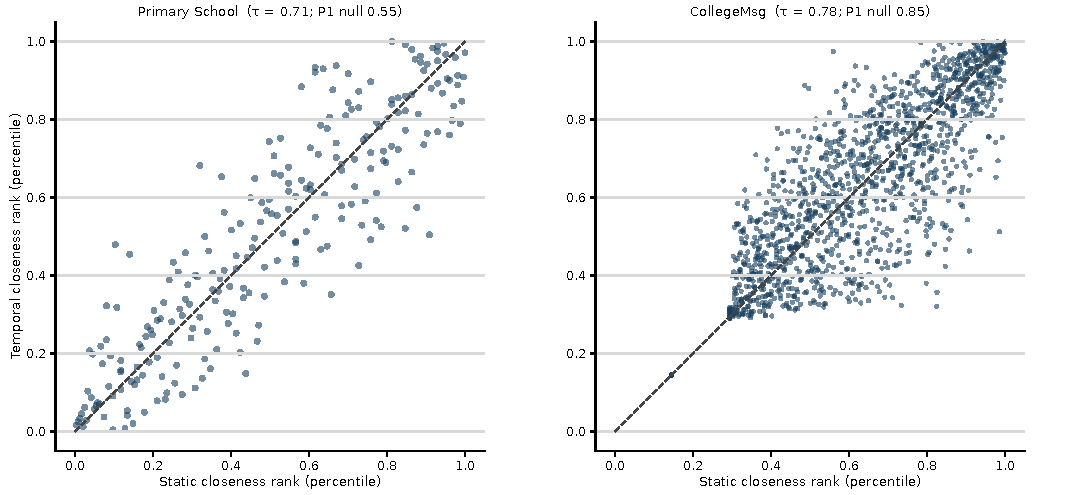
\includegraphics[width=0.8\linewidth]{e_m3b_rank_scatter.pdf}
\caption{Static (unweighted harmonic) vs.\ temporal closeness rank of every node; dashed:
identical rankings. The tied block at the lower left of the CM panel is the 29\% of users
who never send a message.}
\label{fig:m3b}
\end{figure*}

\paragraph{Centrality.}
Static and temporal closeness rankings are clearly correlated in both networks
(\cref{tab:m3b,fig:m3b}; $\tau=0.71$ in PS and $0.78$ in CM, hop distance), so the static
network shows roughly which nodes are central. It is much less reliable about which nodes
are \emph{most} central: only half of the PS top 10\% and two thirds of the CM top 10\%
coincide. In CM the real agreement is somewhat lower than under P1 (0.78 vs.\ 0.85), so
event order makes static closeness a slightly worse guide. The CM $\tau$ is also helped by
the 549 users (29\%) who never send a message and have zero closeness in both rankings
(the tied block in \cref{fig:m3b}).

In PS the effect depends on edge weights. Weighted static closeness agrees poorly with
temporal closeness ($\tau=0.39$, top-10\% overlap 0.29), whereas after P1 the agreement
is high ($0.69\pm0.01$). In the school, most contact weight comes from repeated contacts
within a class during lessons; these happen while the class is already connected and
hardly shorten time-respecting paths to the rest of the school. Under P1 the same contacts
are spread over the day, and a heavy edge becomes a frequent chance to transmit. Without
weights the effect reverses (real 0.71 vs.\ P1 0.55): reaching the school quickly depends
on having many distinct partners, which in PS largely means mixing at breaks.

\emph{Rankings part of H6: partly supported.} The rankings are correlated
($\tau=0.71$--$0.78$) but the top nodes differ by 35--50\%, and in face-to-face data
weighting edges by contact frequency makes the static ranking misleading ($\tau=0.39$).

% Owner: D. Event-started SIR; supersedes the observation-start experiment.
\paragraph{Event-driven SIR (M3c).}\label{sec:d_sir}
Each network uses 200 seeds at randomly selected events in its first 70\% of event
positions. CM seeds use the sender; PS randomly selects either endpoint. The selected
seed event itself is excluded by the strict-time convention. Infectious duration is
fixed, transmission probability is per record, and recovered nodes remain immune.
Final size includes the seed. A major outbreak reaches at least 5\% of period nodes.
Peak delays are averaged over major outbreaks only; $T_{\rm real}/\overline T_{\rm null}$
is a conditional ratio of means. Nulls with no major outbreaks give an undefined peak,
not a zero delay. Simultaneous infections and recoveries are grouped before measuring
prevalence; the earliest maximum is selected.
\begin{table*}[!htbp]\centering\small
\begin{tabular}{@{}llrrrrrrrr@{}}
\toprule & & \multicolumn{3}{c}{Final infected fraction} & \multicolumn{3}{c}{Major outbreak probability} & \multicolumn{2}{c}{Peak ratio} \\
Dataset & $(\beta,D)$ & Real & P1 & P2 & Real & P1 & P2 & vs P1 & vs P2 \\
\midrule
PS & (0.05, 4 h) & 0.629 & 0.776 & 0.823 & 0.860 & 0.908 & 0.920 & 1.160 & 1.214 \\
PS & (0.02, 4 h) & 0.373 & 0.420 & 0.559 & 0.700 & 0.754 & 0.778 & 1.000 & 1.088 \\
PS & (0.1, 4 h) & 0.734 & 0.893 & 0.918 & 0.910 & 0.960 & 0.973 & 1.311 & 1.340 \\
PS & (0.05, 1 h) & 0.373 & 0.634 & 0.674 & 0.745 & 0.844 & 0.852 & 1.021 & 1.265 \\
CM & (0.2, 336 h) & 0.256 & 0.250 & 0.276 & 0.825 & 0.791 & 0.799 & 0.888 & 0.995 \\
CM & (0.05, 336 h) & 0.026 & 0.013 & 0.025 & 0.215 & 0.082 & 0.192 & 0.934 & 0.991 \\
CM & (0.5, 336 h) & 0.460 & 0.506 & 0.530 & 0.975 & 0.954 & 0.965 & 0.924 & 0.982 \\
CM & (0.2, 72 h) & 0.074 & 0.043 & 0.066 & 0.555 & 0.342 & 0.428 & 0.720 & 1.013 \\
\bottomrule\end{tabular}
\caption{Four SIR settings per dataset, 200 seeds per network, 20 nulls per family.
The first setting in each dataset is primary. The peak-ratio population is restricted
to major outbreaks and can differ between real and null networks.}\label{tab:d-sir}
\end{table*}
\begin{figure*}[!htbp]
\centering
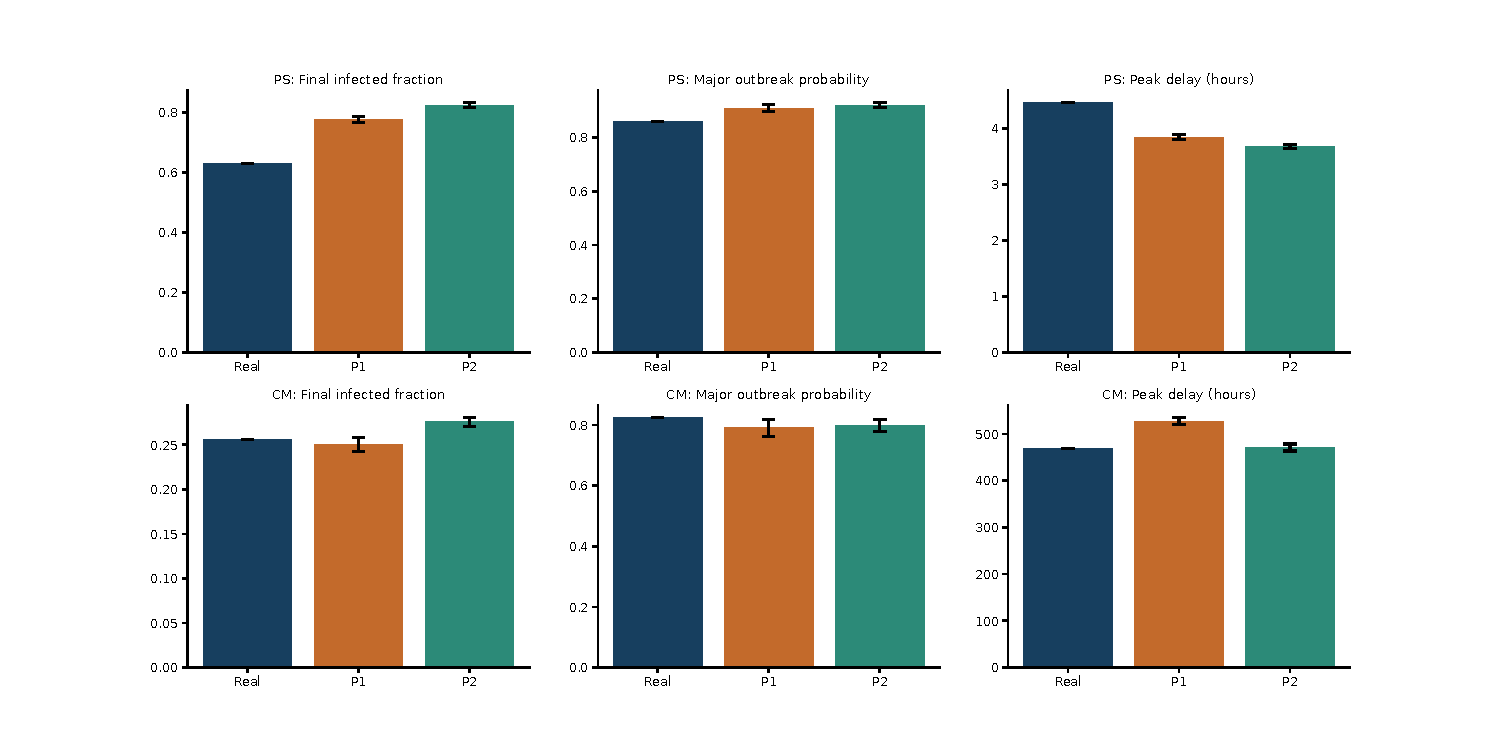
\includegraphics[width=\linewidth]{d_sir_event_seeds.pdf}
\caption{Primary SIR settings. Peak delay is conditional on major outbreaks; errors describe null-network variation.}
\label{fig:d_sir}
\end{figure*}
The revised design produces nontrivial CM outbreaks. Absence of secondary infections
in the earlier run arose from infecting seeds at the observation boundary with an
unsuitable short duration; it is not evidence for an intrinsic property of CM.

\paragraph{Parameter, null and outcome dependence.}
For PS versus P1, the peak ratio is 1.0005 at $\beta=.02$ (negligible peak difference),
1.160 at .05 and 1.311 at .10 for a four-hour infectious duration. Final size is
lower than both null families in all four tested settings; at the primary setting
it is 0.629 versus P1 0.776. The qualifying populations also differ: major outbreaks
occur for 0.860 of real seeds versus a mean 0.908 under P1. Conditional peak comparisons
therefore use different seed subsets and are not paired-seed causal slowdowns.

CM peaks earlier than P1 across the full-period settings (ratios 0.72--0.94),
whereas P2 peak ratios are approximately 0.98--1.01. Even the choice of timing
metric matters: at $\beta=.5$, 14 days, the peak ratio to P1 is 0.924 but the
half-final-size time ratio is 1.061. The latter is time to half of each trajectory's
own final infected count, not time to a common epidemic size. These opposing signs
exclude a general claim that the entire spreading process is faster or slower.
In CM's second half, two weaker settings have no major real outbreaks (undefined
peak ratios); the primary setting still has major-outbreak probability 0.360.

PS's real mean final fraction is 0.629 over the full interval versus 0.821/0.788
in the halves. Uniform sampling from the first 70\% of each event stream changes
seed identities, start positions and residual observation horizons when the interval
is split. Finite horizons and schedule boundaries may contribute; these CSV comparisons
alone do not identify their contribution separately. These are protocol sensitivities,
not evidence that truncating the data intrinsically strengthens propagation.

\paragraph{Verdict on H6 and H7.}
H6's reachability component is supported under the multi-start protocol in both datasets;
rankings show a partial effect, with correlated rankings but different top nodes.
H7 is conditional on parameters and the reference model. PS peaks later under its
primary setting; CM peaks earlier than P1 across the four tested full-period settings and is close
to P2. The claim that slowing is strongest in CM is therefore not supported.
Peak timing among major outbreaks does not by itself measure population-wide epidemic speed.

\subsection{CIT model diagnostics and robustness}
\label{sec:b-diagnostics}
% Owner: B. All diagnostics use the completed CIT run, not new experiments.
\paragraph{Null controls and ageing alternatives.}
\Cref{fig:growth}(b) shows the observed exponent and both null ensembles;
\cref{tab:b-age-models} reports the age-kernel comparison without a duplicate AIC plot.
P3b matches mean citation age because its age weights were fitted to these data;
that agreement is a property of the control, not independent evidence for ageing.
With only 20 realizations per null, an observed value above all nulls has empirical
one-sided probability $1/21$; this does not justify a precise tail estimate.
The ageing comparison is on identical risk sets and observations.

\begin{table}[t]
\centering\small
\begin{tabular*}{\columnwidth}{@{\extracolsep{\fill}}lrr@{}}
\toprule
Age kernel & Parameters & $\Delta$AIC\\
\midrule
Lognormal & 2 & 0.0\\
Exponential & 1 & 537.8\\
Power-law & 1 & 9,360.5\\
Uniform & 0 & 41,796.7\\
\bottomrule
\end{tabular*}
\caption{CIT age-preference alternatives on common observed support. AIC selects
among the declared models, not among every possible ageing mechanism.}
\label{tab:b-age-models}
\end{table}



\paragraph{Fit quality does not establish predictability.}
The full-history sample is 500 of 1,019 papers with at least ten citations by age
15; the forecast sample is 500 of 1,220 eligible papers selected only by having
at least five citations in their first five years. Both samples are drawn with a
fixed seed. Median full-history RMSLE is 0.0736 and median scaled-collapse RMSE
0.0220 (90th percentile 0.0453); 10.2\% of full-history fits hit a parameter bound.
These are in-sample diagnostics. Held-out scoring in
\cref{tab:b-forecast} and \cref{fig:b-wsb-validation} provides the separate
predictive test. All 500 short-history optimizations report success, while
193 touch a bound; these are distinct diagnostics. In particular, a collapse
obtained using parameters fitted to
the same curve is not independent evidence for universal citation dynamics.



\begin{table}[t]
\centering\small
\setlength{\tabcolsep}{4pt}
\begin{tabular*}{\columnwidth}{@{\extracolsep{\fill}}llrr@{}}
\toprule
Target & Model & MAE & RMSLE\\
\midrule
15 yr & WSB & 15.144 & 0.601\\
 & Linear & 17.064 & 0.662\\
 & No-age PA & 27,588 & 4.601\\
\midrule
2020 & WSB & 28.016 & 0.778\\
 & Linear & 27.271 & 0.876\\
 & No-age PA & $2.79\!\times\!10^6$ & 7.000\\
\bottomrule
\end{tabular*}
\caption{Matched forecasts on 500 selected papers using only years 1--5 for
training. Age 15 is fully observed for the selected cohort and is the primary fixed
ten-year-ahead task; 2020 is a secondary, variable-horizon within-corpus total.
The exponential no-age PA baseline over-extrapolates; beating it alone is a weak
test. The paired MAE intervals against linear both include zero.}
\label{tab:b-forecast}
\end{table}

\paragraph{Sensitivity of the conclusions.}
\Cref{tab:b-robustness} reports time splits, cutoff and corpus-selection checks.
The sign of degree preference and superlinear full-period growth persist, but
$a$ is substantially weaker in the late period. Degree offsets 0.5 and 2 give
$\alpha=0.604$ and 0.858, so the numerical exponent is convention-dependent.
Including 5,486 year ties gives $a=1.324$; ties remain excluded from the primary
DAG. Effective-diameter endpoint estimates remain 6 hops with 64, 128 or 256
sources. First-ten versus all-twenty null means of $\alpha$ are 0.00055/0.00059
(P3a) and $-0.65320$/$-0.65118$ (P3b).
Lognormal ageing is preferred in all target cohorts and both observation halves,
but the recent cohort's fitted tail extends beyond its observed follow-up.
These checks support qualitative stability without eliminating coverage bias,
right censoring or unobserved fitness.

\begin{table}[t]
\centering\small
\begin{tabular*}{\columnwidth}{@{\extracolsep{\fill}}lrr@{}}
\toprule
Variant & $\alpha$ & $a$\\
\midrule
1990--2020 (primary) & 0.714 & 1.343\\
1990--2004 & 0.684 & 1.455\\
2005--2020 & 0.721 & 1.065\\
Cutoff 2015 & 0.722 & 1.427\\
Core venue families & 0.731 & 1.410\\
Same-year edges included & -- & 1.324\\
\bottomrule
\end{tabular*}
\caption{CIT robustness from the saved run. Core venue families contain 14,235
nodes and 47,009 primary edges; the year-tie variant is structural only.}
\label{tab:b-robustness}
\end{table}

\subsection{Observation and null-count sensitivity}\label{sec:r-robustness}
\begin{table}[!htbp]\centering\small
\begin{tabular*}{\columnwidth}{@{\extracolsep{\fill}}llrrrr@{}}
\toprule & Measure & Full & First & Second & 60 nulls \\
\midrule
PS & H1 density & 3.359 & 2.596 & 2.487 & -- \\
CM & H1 density & 3.862 & 3.623 & 3.478 & -- \\
PS & H1 clustering & 1.628 & 0.921 & 0.959 & -- \\
PS & H2 $\Delta B$ & 0.016 & 0.116 & 0.120 & 0.016 \\
CM & H2 $\Delta B$ & 0.336 & 0.381 & 0.313 & 0.336 \\
PS & H3 $\Delta J$ & -0.147 & -0.192 & -0.184 & -0.147 \\
CM & H3 $\Delta J$ & 0.027 & -0.039 & -0.022 & 0.027 \\
PS & H6 $R$ & 0.866 & 0.815 & 0.765 & 0.866 \\
CM & H6 $R$ & 0.205 & 0.314 & 0.177 & 0.205 \\
PS & H7 ratio P1 & 1.160 & 1.081 & 1.095 & 1.161 \\
CM & H7 ratio P1 & 0.888 & 0.856 & 0.865 & 0.884 \\
PS & H7 ratio P2 & 1.214 & 1.142 & 1.160 & 1.212 \\
CM & H7 ratio P2 & 0.995 & 0.961 & 0.877 & 0.999 \\
PS & H5 NMI & 0.816 & 0.812 & 0.818 & 0.816 \\
CM & H5 NMI & 0.519 & 0.374 & 0.663 & 0.519 \\
CIT & H4 $\alpha$ & 0.714 & 0.684 & 0.721 & 0.714 \\
\bottomrule\end{tabular*}
\caption{Elapsed-time halves for PS/CM and analysis-year halves for CIT. A uses no null.
The 60-null run nests the first 20; H7 ratios condition on major outbreaks. A and E real
values do not depend on null count, while H2/H3 differences and H7 ratios do. H2/H3 are real minus P1; H5/H6 show observed NMI/$R$, and H7 shows conditional ratios.}\label{tab:robust-halves}
\end{table}
Primary H7 ratios remain on the same side of one under the 20/60 comparison:
PS changes from 1.160 to 1.161 and CM from 0.888 to 0.884. Both primary half-period
ratios preserve those directions. This does not hold uniformly over parameter settings:
at PS $\beta=.02$, $D=4$ h the full-period ratio moves from 1.0005 (20 nulls) to
0.9992 (60 nulls), so no directional slowing claim is supported there. PS's one-hour
setting peaks earlier than P1 in the first half (ratio 0.874) despite a full-period
ratio above one. In CM's second half, two settings produce no major real outbreaks
and their conditional peak ratios are undefined; these are not treated as zero.
The primary CM setting remains defined in that half (major-outbreak probability 0.360).
CM's H3 contrast reverses from $+0.027$ in the full interval to $-0.039/-0.022$
in the halves. PS's H2 excess grows from 0.016 to 0.116/0.120, while its clustering
sensitivity drops from 1.628 to 0.921/0.959. These are substantive interval
sensitivities even when increasing the null ensemble from 20 to 60 changes little.
Individual realizations, sample SDs and 20/60 changes are retained in the supplementary
CSV files. Splitting changes node populations and the time available for paths and
outbreaks, so agreement of signs is more informative than equality of raw effect sizes.
The established E resolution grid is retained. CIT retains its original history for
PA exposure and eligible targets; its diameter is measured on cumulative endpoint
graphs. WSB uses the original age-15 forecast test, additionally stratified by early
and late publication cohorts, rather than being treated as a stationary half-window test.

\subsection{Cross-network summary}\label{sec:r-cross}
\Cref{tab:cross} reports the time-effect measure of each hypothesis together with the
verdict reached in the preceding subsections. The measures differ in units and
interpretation, so the table does not define a common sensitivity score for a network type.
Temporal information is essential for every hypothesis in at least one network, but the
direction and robustness of the effect vary with the system and, for H2, H3 and H7, with the
event definition, window width, observation interval or reference model.

\begin{table*}[t]
\centering\small
\setlength{\tabcolsep}{4pt}
\begin{tabularx}{\textwidth}{@{}llrrr>{\raggedright\arraybackslash}X@{}}
\toprule ID & Measure & PS & CM & CIT & Verdict \\
\midrule
H1 & Density sensitivity & 3.262 & 5.411 & 1.798 & Supported in all three networks \\
H2 & $\Delta B$ vs P1 & 0.016 & 0.336 & -- & Burstiness supported in CM; small and definition-dependent in PS; memory not supported \\
H3 & $\Delta J$ vs P1 & $-0.147$ & 0.027 & -- & Turnover supported in PS; CM persistence depends on width and interval \\
H4 & $\Delta\alpha$ vs P3a & -- & -- & 0.713 & Attachment, ageing and densification supported; no diameter shrinkage or forecast advantage \\
H5 & $\Delta$ adjacent NMI vs P1 & $-0.096$ & 0.098 & -- & Supported in PS; not supported in CM \\
\multirow{2}{*}{H6} & $\Delta R$ vs P1 & $-0.134$ & $-0.120$ & -- & \multirow{2}{=}{Reachability restricted in both; rankings correlated but top nodes differ} \\
 & $\Delta R$ vs P2 & $-0.134$ & $-0.031$ & -- & \\
\multirow{2}{*}{H7} & Peak ratio vs P1 & 1.160 & 0.888 & -- & \multirow{2}{=}{Conditionally supported in PS; not supported in CM} \\
 & Peak ratio vs P2 & 1.214 & 0.995 & -- & \\
\bottomrule\end{tabularx}
\caption{Time effects and verdicts. H1 is descriptive and uses different window grids per
network (PS 5\,min--24\,h, CM 1\,h--30\,d, CIT 1--10 years), so its values cannot be ranked.
H5 uses 15-min (PS) and 7-day (CM) windows. H7 reports the primary SIR setting and
conditions on major outbreaks. A dash denotes inapplicability and not a zero effect.}
\label{tab:cross}
\end{table*}



%=====================================================================
\section{Discussion}
\label{sec:discussion}

\paragraph{What the static network already tells us.}
Conclusions that survive aggregation can be read from \cref{tab:cross}.
For CIT, the final aggregate describes degree heterogeneity, clustering and
connected components. It cannot by itself identify preferential attachment or
ageing: these compare new citations with prior degrees and paper ages.
Even densification requires a sequence of historical $N(t),E(t)$ pairs, rather
than one final graph. For PS and CM, static aggregation preserves the
existence of links but hides their timing, repetition and turnover.

\paragraph{What requires time.}
Some conclusions need windows (Parts I and III) and others the full event order
(Parts II and IV).
For H2, both PS and CM exhibit higher pooled burstiness than their P1
timestamp-shuffled baselines. The excess is relatively small for PS
($+0.0163$) but much larger for CM ($+0.3361$).
However, observed memory is lower than P1 in both networks,
so stronger-than-null positive memory is not supported.
For H3, adjacent-window link overlap also differs from the
randomized baseline, demonstrating that static aggregation
cannot capture temporal link turnover.
Community reorganisation, time-respecting reachability and
spreading speed additionally require temporal information,
although their conclusions depend on the corresponding analyses.

\paragraph{Why network types differ.}
The three networks differ in generating mechanism (physical proximity, voluntary
messaging, citing earlier work), time scale and edge semantics (a contact ends, a
message is a point event, a citation persists).
PS interactions are constrained by school schedules and physical proximity,
whereas CM records voluntary online communication over a much longer period.
These differences may contribute to the stronger excess burstiness in CM.
For H3, PS has lower adjacent-hour Jaccard similarity than P1
($0.2198$ versus $0.3668$), while CM has higher adjacent-week
similarity ($0.0958$ versus $0.0691$).
However, the CM contrast reverses at a 14-day window.
Thus, temporal persistence depends on both network type and
aggregation scale, rather than following a universal pattern.
CIT has persistent edges and measured age-dependent target preferences.
Direct comparisons remain conditional on differences in event definitions
and observation periods.

\paragraph{Robustness.}
We check the choice of window size, the observation period (first vs.\ second
half), the community-detection resolution and the choice of null model.
For H2, PS was evaluated using both raw 20-second contact records
and merged contact episodes. Both definitions produce higher
burstiness and lower memory than P1, although the excess
burstiness changes from $+0.1020$ to $+0.0163$.
For H3, PS shows lower link overlap than P1 across all four
tested windows, while CM changes from higher to lower overlap
as the window increases to 14 days.
The P2b endpoint-swap implementation passes structural invariant
checks, but its mixing behaviour has not been fully assessed.

For CIT, the full-period densification exponent is 1.343 but falls to 1.065 in
the later half, while remaining 1.427 with cutoff 2015. Positive degree preference
persists under all declared variants, although its exponent depends on the degree
offset. The diameter verdict is unchanged by the sampled-source sensitivity
checks. These are qualitative robustness findings, not evidence that coverage
and censoring have been removed.

% Owner: B (measured citation-specific interpretation).
\paragraph{Citation-specific evidence.}
CIT supports degree preference and age-dependent target choice, but separates two
claims often grouped together: cumulative edges grow superlinearly, while the
sampled effective diameter does not shrink. A three-parameter citation curve
fits selected histories well, yet its paired MAE advantage over linear prediction
is unresolved. Annual zero clustering is imposed by the strict-year snapshot
construction. These examples show why representation, fitted-sample description
and held-out prediction require separate interpretations. Late reference coverage,
within-venue selection and right censoring constrain all citation conclusions.

\paragraph{Limitations.}
There is one dataset per network type, so generality is limited and conclusions
hold ``in these data''. For PS and CM, pooled burstiness and memory
may be influenced by heterogeneous edge activity.
P1 preserves the global timestamp distribution and therefore does
not eliminate all temporal nonstationarity.
The short PS observation period also introduces boundary effects
in edge-lifetime measurements.
Window-based Jaccard similarity depends on the chosen aggregation scale.
Although P2b preserves event participation counts, its endpoint swaps
are not guaranteed to sample uniformly from all admissible networks.
The 20-draw null ensembles give coarse tail resolution.

CIT also has within-venue sampling, annual timestamp ties and changing reference
coverage. Its year-block bootstrap intervals are descriptive; cumulative graph
observations are dependent.
Forecast selection excludes low-cited papers, and 38.6\% of short-history WSB fits
hit parameter bounds despite optimizer success in every case; fitted collapse
is not independent validation. The primary age-15 target is fully observed,
whereas 2020 endpoint comparisons mix forecast horizons. Neither removes
within-venue citation-coverage limitations.
Boundary effects and sampling bias remain (finite two-day contact window,
sensor participation).
Citation networks are degenerate temporal networks (DAG, no deletion), which is
why several methods do not apply. Each system also contains several time scales
\citep{holme2015modern}, so a window that suits one process may hide another.
Finally, SocioPatterns data are released under CC BY-NC-SA.

%=====================================================================
\section{Conclusion}
\label{sec:conclusion}
This study tested seven hypotheses from the temporal-network literature on a contact, a
messaging and a citation network within a common framework. The importance of temporal
information depends on the question asked. In the citation network, the final aggregate
describes degree heterogeneity and connectivity, whereas preferential attachment, ageing
and the growth law require historical degrees, publication ages or cumulative snapshots.
Within the selected AMiner corpus, sublinear degree preference and age-dependent citation
choice coexist with superlinear edge growth, but the sampled effective diameter does not
shrink. The WSB model describes citation histories compactly without an established
forecast advantage over linear extrapolation, so descriptive fit, temporal mechanism and
predictive value must be assessed separately.

In the contact and messaging networks, structural metrics depend strongly on the window
width, and time ordering restricts reachability over a finite horizon. Burstiness exceeds
the timestamp-shuffled baseline robustly in CM, whereas in PS the excess is small and depends
on the observation interval and the event definition; memory is weaker than under the
baseline in both networks. The persistence of CM ties relative to the baseline reverses
within both observation halves and at 14-day windows. Static communities conceal the midday
mixing in PS, while CM shows no comparable reorganisation. Conditional on major outbreaks,
epidemic peaks in PS occur later than under both reference models at the primary setting,
whereas CM does not support a general slowdown. These hypothesis-specific effects cannot be
combined into a single ranking of network types without further assumptions. Several
datasets per network type, broader corpus coverage, finer-resolution citation dates and
predictive tests under alternative censoring assumptions would strengthen the conclusions.


{\small
\bibliographystyle{ieeenat_fullname}
\bibliography{references}
}

\end{document}
